%%%%%%%%%%%%%%%%%%%%%%%%%%%%%%%%%%%%%%
\documentclass[final,table,xcdraw,hyperref={pdfpagelabels=false}]{beamer}
\usepackage{grffile}
\mode<presentation>{\usetheme{I6pd2}}
\usepackage[english]{babel}
\usepackage[latin1]{inputenc}
\usepackage{amsmath,amsthm, amssymb, latexsym}
%\usepackage{times}\usefonttheme{professionalfonts}  % obsolete
%\usefonttheme[onlymath]{serif}
\boldmath
% \documentclass[final]{beamer}
% \usepackage{color}
\usepackage[orientation=portrait,size=a1,scale=1.4,debug]{beamerposter}
% \usepackage[size=a0llarg,orientation=portrait]{beamerposter}
\usepackage{graphicx}			% allows us to import images
\usepackage{multirow} 
\usepackage{tabularx} 
\usepackage{setspace}
\usepackage{booktabs}
\usepackage{listings}
\usepackage{xcolor}



\definecolor{lightgray}{rgb}{.8,.8,.8}
\definecolor{darkgray}{rgb}{.4,.4,.4}
\definecolor{purple}{rgb}{0.65, 0.12, 0.82}

\lstdefinelanguage{SVGscript}{
  keywords={Create, Move, Modify, Source, Destroy, Rotate, Scale},
  keywordstyle=\color{brown}\bfseries,
  ndkeywords={func, endfunc, if, endif, while, endwhile, call, return},
  ndkeywordstyle=\color{blue}\bfseries,
  classoffset=2,
  morekeywords={Circle,Text,Rectangle},
  keywordstyle=\color{magenta}\bfseries,
  classoffset=0,
  identifierstyle=\color{black},
  sensitive=true,
  comment=[l]{//},
  morecomment=[s]{/*}{*/},
  commentstyle=\color {green}\ttfamily,
  stringstyle=\color{red}\ttfamily,
  morestring=[b]',
  morestring=[b]"
}

\lstset{
   language=SVGscript,
   %backgroundcolor=\color{white},
   extendedchars=true,
   %basicstyle=\fontfamily{pcr}\selectfont\footnotesize\color{blue}\footnotesize,
   basicstyle=\footnotesize\ttfamily\color{blue},
   showstringspaces=false,
   showspaces=false,
   %numbers=false
   %numberstyle=\footnotesize\color{darkgray},
   numbersep=2pt,
   tabsize=2,
   breaklines=true,
   showtabs=false,
   captionpos=b
}

\newcommand{\leftfoot}{http://nlp.cs.upc.edu/freeling} % Left footer text
\newcommand{\rightfoot}{TALP Research Center 2018} % Right footer text

%-----------------------------------------------------------
% Define the column width and poster size
% To set effective sepwid, onecolwid and twocolwid values, first choose how many columns you want and how much separation you want between columns
% columns = 2
% sepwid = 0.024
% onecolwid = (1-(2+1)*0.024)/2 = 0.464
% twocolwid = oncolwid*2 + sepwid = 0.952
% The separation I chose is 0.024 and I want 4 columns
% Then set onecolwid to be (1-(4+1)*0.024)/4 = 0.22
% Set twocolwid to be 2*onecolwid + sepwid = 0.464
%-----------------------------------------------------------

\newlength{\sepwid}
\newlength{\onecolwid}
\newlength{\twocolwid}
% \setlength{\paperwidth}{36in}
% \setlength{\paperheight}{48in}
\setlength{\sepwid}{0.002\paperwidth}
\setlength{\onecolwid}{0.468\paperwidth}
\setlength{\twocolwid}{0.960\paperwidth}
% \setlength{\topmargin}{-0.5in}
% \usetheme{emiliposter}
% \usetheme{Icy}
%-----------------------------------------------------------
% Define colours (see beamerthemeconfposter.sty to change the colour definitions)
%-----------------------------------------------------------

%-----------------------------------------------------------
% Name and authors of poster/paper/research
%-----------------------------------------------------------

\title{Disability annotation on documents from the biomedical domain}
\author{Pol Alvarez Vecino$^{\ast}$, Llu�s Padr�$^{\dagger}$}
\institute{$^{\ast}$Barcelona Supercomputing Center. Barcelona, Spain. \texttt{pol.alvarez@bsc.es}\\
         $^{\dagger}$TALP Research Center. Universitat Polit�cnica de Catalunya. Barcelona, Spain. \texttt{padro@cs.upc.edu}}

%-----------------------------------------------------------
% Start the poster itself
%-----------------------------------------------------------
% The \rmfamily command is used frequently throughout the poster to force a serif font to be used for the body text
% Serif font is better for small text, sans-serif font is better for headers (for readability reasons)
%-----------------------------------------------------------

\begin{document}

\begin{small}
\begin{frame}[t,fragile]

\begin{columns}[t] % the [t] option aligns the column's content at the top
\begin{column}{\sepwid}\end{column} % empty spacer column

\begin{column}{\twocolwid}
\begin{block}{\vspace{-0.3cm} Abstract}

This paper describes the UPC\_2 system participation in DIANN (\textit{Disability annotation on documents from the biomedical domain}) shared task, framed in the IBEREVAL 2018 evaluation workshop\footnote{\texttt{http://nlp.uned.es/diann}}.
The system tackles the detection of disabilities using a CRF to perform IOB Named Entity Recognition (NER). Regarding the detection of negated disabilities, the out-of-the-box NegEx rule-based system is used.
\keywords{Medical Named Entity Recognition \and CRF \and Disabilities \and Negation detection}

\end{block}
\end{column}

\begin{column}{\sepwid}\end{column} % empty spacer column

\end{columns}


\begin{columns}[t] % the [t] option aligns the column's content at the top
\begin{column}{\sepwid}\end{column} % empty spacer column

\begin{column}{\onecolwid}

\begin{block}{\vspace{-0.3cm} 1. Introduction: Task}

\begin{itemize}
\item \textbf{Annotate disabilities} and their \textbf{negation} on documents from the biomedical domain.
\item Input: \textbf{short texts} with the disabilities and negations \textbf{tagged with XML}.
\item Simple disability annotation:
\lstset{language=XML}
\begin{lstlisting}
... reliability of the MCA in Spanish to identify <dis>mild cognitive impairment</dis> (<dis>MCI</dis>)...
\end{lstlisting}

\item Negated disability annotation:
\begin{lstlisting}
... <scp> <neg>without</neg> <dis>dementia</dis> </scp>, significant differences were obtained in terms ...
\end{lstlisting}
\end{itemize}
\end{block}

\begin{block}{\vspace{-0.3cm} 2. Approach}
\begin{itemize}
    \item The approach to the problem was to solve it in two steps:
    \bigskip
    \item \textbf{Disabilities:}
    \medskip
    \begin{itemize}
        \item Convert all words into tuples: \textit{(word, POS, IOB-tag)}.
        \item Use Conditional Random Fields (CRF) to predict the disability IOB-tags.
        \item Convert IOB-tags to sentences/disabilities.
    \end{itemize}
    \item \textbf{Negation:}
    \medskip
    \begin{itemize}
	    \item Feed each tuple sentence/disability to a negation software. 
        \item Filter out the probable false positives.
        \item Convert input back again into XML tagged files.
    \end{itemize} 
\end{itemize} 
\end{block}

\begin{block}{\vspace{-0.3cm} 3. Creating the training data}
  \begin{figure}\centering
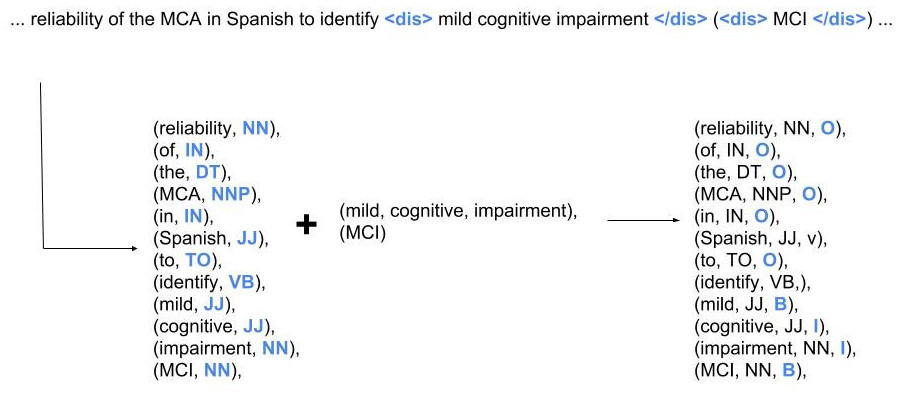
\includegraphics[width=0.95\textwidth]{images/diann_disabilities.jpg}
\caption{Pipeline to create the training data for the CRF model.}
\end{figure}
\end{block}


\begin{block}{\vspace{-0.3cm} 4. CRF Model \& Features}

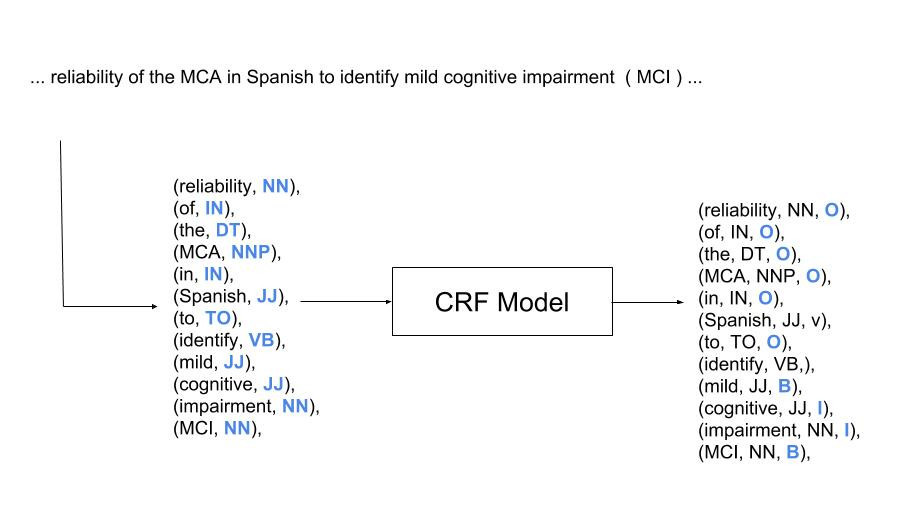
\includegraphics[width=0.95\textwidth]{images/Test_diann_disabilities.jpg}

%  Once the data in is $(word, pos, iob)$-format the next step is to decide which features are going to be used to train the CRF model.
\bigskip


\textbf{Groups of features:}
 

\begin{itemize}
\item 1. Derived from the \textbf{curent word} like word, POS, lemma or all-caps.
\medskip
\item 2. Build from \textbf{entitites/acronyms lists} such as  is-acronym.
\medskip
\item 3. Derived from the \textbf{previous/next words} like word, POS, or lemma.
\medskip
\item 4. Concatenation of \textbf{current word's feature and next/previous'} one.
\item 5. Concatenation of the \textbf{two previous/next} words' features.
\end{itemize}
\end{block}

\end{column}

\begin{column}{\sepwid}\end{column} % empty spacer column

\begin{column}{\onecolwid}

\begin{block}{\vspace{-0.3cm} 5. CRF Model: Training}
\begin{itemize}
\item Feature Selection\footnote{All validation results use 10-fold cross-validation}:
  \begin{itemize}
  \item Start with all groups activated and with all features per group
  \item Deactivate a group and check if precision increases/decrease
  \item If precision increases:
    \begin{itemize}
    \item Reactivate the group
    \item Deactivate each feature of the group and reactivate it only if precision decreases
    \end{itemize}
  \item If precision decreases just remove the group from the feature's set
  \end{itemize}
\item Lists' Creation:
  \begin{itemize}
  \item During model evaluation, entities/acronyms lists are created out of the training fold
  \item Once the model is chosen, built the lists with all the training data
  \end{itemize}
\end{itemize}
\end{block}


\begin{block}{\vspace{-0.3cm} 6. Negation Detection}
 \begin{figure}\centering
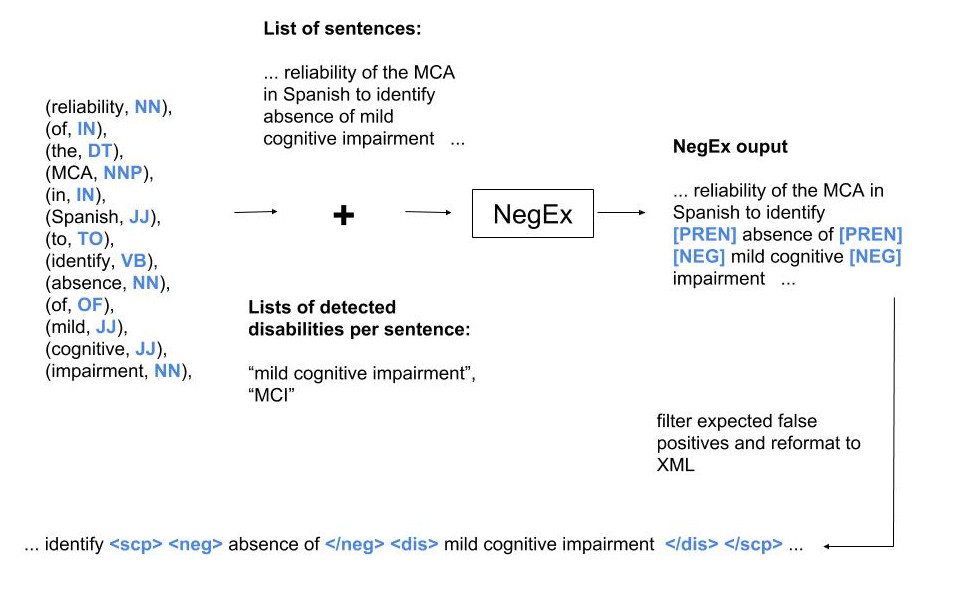
\includegraphics[width=0.95\textwidth]{images/Negex_diann_disabilities.jpg}
\caption{Pipeline to tag negated phrases and final XML formatting.}
\end{figure}
 
\end{block}


\begin{block}{\vspace{-0.3cm} 7. Experiments and Results}

\begin{table}[]
\centering
\begin{tabular}{|lccc|ccc|}
\hline
\multicolumn{1}{|l|}{}                                                         & \multicolumn{3}{l|}{\cellcolor[HTML]{CADFF6}Spanish}                                                                                       & \multicolumn{3}{l|}{\cellcolor[HTML]{CADFF6}English}                                                                                        \\ \cline{2-7} 
\multicolumn{1}{|l|}{}                                                         & \multicolumn{1}{c|}{Precision}               & \multicolumn{1}{c|}{Recall}                  & \multicolumn{1}{c|}{F1 score}                & \multicolumn{1}{c|}{Precision}               & \multicolumn{1}{c|}{Recall}                  & F1 score                                      \\ \hline
\rowcolor[HTML]{EEEEEE} 
\multicolumn{7}{|l|}{Group disabled: 2}\\ \hline
\multicolumn{1}{|l|}{\cellcolor[HTML]{CADFF6}Negation}                         & 0.50                                       & 0.55                                        & 0.52   
    & 0.46                                        & 0.35                                        & 0.40                                          \\
\multicolumn{1}{|l|}{\cellcolor[HTML]{CADFF6}Disability}                                                          & 0.72                                        & 0.63                                        & \textbf{0.68} & 0.72                                        & 0.58                                        & 0.64                                          \\
\rowcolor[HTML]{EEEEEE} 
\multicolumn{7}{|l|}{Group disabled: 3}\\ \hline
\multicolumn{1}{|l|}{\cellcolor[HTML]{CADFF6}Negation}                       & 0.50                                        & 0.50                                        & 0.50                                        & \textbf{0.48}                                        & 0.35                                       & 0.41                                        \\
\multicolumn{1}{|l|}{\cellcolor[HTML]{CADFF6}Disability}               & 0.73                                        & 0.51                                        & 0.60                                        & \textbf{0.75}                                        & 0.56                                        & 0.64                                         \\
\rowcolor[HTML]{EEEEEE} 
\multicolumn{7}{|l|}{Group disabled: 4}\\ \hline
\multicolumn{1}{|l|}{\cellcolor[HTML]{CADFF6}Negation}                       & 0.51                                        & \textbf{0.58}                                        & \textbf{0.54}                                        & \textbf{0.48}                                        & 0.40                                        & \textbf{0.44} \\
\multicolumn{1}{|l|}{\cellcolor[HTML]{CADFF6}Disability}               & \textbf{0.74}                                        & 0.59                                        & 0.65                                        & 0.74                                        & 0.65                                        & 0.70                                         \\
\rowcolor[HTML]{EEEEEE} 
\multicolumn{7}{|l|}{Group disabled: 5}\\ \hline
\multicolumn{1}{|l|}{\cellcolor[HTML]{CADFF6}Negation}                       & 0.51                                        & 0.55                                        & 0.53                                        & \textbf{0.48}                                        & 0.38                                        & 0.42                                         \\
\multicolumn{1}{|l|}{\cellcolor[HTML]{CADFF6}Disability}               & 0.71                                        & 0.59                                        & 0.64                                        & \textbf{0.75}                                        & 0.65                                        & 0.69                                         \\
\rowcolor[HTML]{EEEEEE} 
\multicolumn{7}{|l|}{Group disabled: None}\\ \hline
\multicolumn{1}{|l|}{\cellcolor[HTML]{CADFF6}Negation}                       & \textbf{0.52}                              & 0.55                                        & 0.53                                        & 0.47                                        & \textbf{0.41}                                        & 0.43                                         \\
\multicolumn{1}{|l|}{\cellcolor[HTML]{CADFF6}Disability}               & \textbf{0.74}                                        & 0.62                                        & \textbf{0.68}                                        & \textbf{0.75}                                        & \textbf{0.67}                                        & \textbf{0.71}                                         \\ \hline
\end{tabular}
\medskip
\caption{Results of cross-validation experiments deactivating one feature group at a time.}
\label{tab:xval-results}
\end{table}



% TESTING FINAL RESULTS FULL FEATURES

\begin{table}[]
\centering
\begin{tabular}{|lccc|ccc|}
\hline
\multicolumn{1}{|l|}{}                                                         & \multicolumn{3}{l|}{\cellcolor[HTML]{CADFF6}Exact Match}                                                                                   & \multicolumn{3}{l|}{\cellcolor[HTML]{CADFF6}Partial Match}                                                                                  \\ \cline{2-7} 
\multicolumn{1}{|l|}{}                                                         & \multicolumn{1}{c|}{Precision}               & \multicolumn{1}{c|}{Recall}                  & \multicolumn{1}{c|}{F1 score}                & \multicolumn{1}{c|}{Precision}               & \multicolumn{1}{c|}{Recall}                  & F1 score                                      \\ \hline
\rowcolor[HTML]{EEEEEE} 
English                                                                        & \multicolumn{1}{l}{\cellcolor[HTML]{EEEEEE}} & \multicolumn{1}{l}{\cellcolor[HTML]{EEEEEE}} & \multicolumn{1}{l}{\cellcolor[HTML]{EEEEEE}} & \multicolumn{1}{l}{\cellcolor[HTML]{EEEEEE}} & \multicolumn{1}{l}{\cellcolor[HTML]{EEEEEE}} & \multicolumn{1}{l|}{\cellcolor[HTML]{EEEEEE}} \\ \hline
\multicolumn{1}{|l|}{\cellcolor[HTML]{CADFF6}Disability}                       & 0.756                                        & 0.560                                        & 0.643                                        & 0.822                                        & 0.588                                        & 0.686                                         \\
\multicolumn{1}{|l|}{\cellcolor[HTML]{CADFF6}Negated Disability}               & 0.647                                        & 0.478                                        & 0.550                                        & 0.941                                        & 0.696                                        & 0.800                                           \\
\multicolumn{1}{|l|}{\cellcolor[HTML]{CADFF6}Non-negated + Negated Disability} & 0.724                                        & 0.519                                        & 0.604                                        & 0.822                                        & 0.588                                        & 0.686                                         \\ \hline
\rowcolor[HTML]{EEEEEE} 
Spanish                                                                        &                                              &                                              &                                              &                                              &                                              &                                               \\ \hline
\multicolumn{1}{|l|}{\cellcolor[HTML]{CADFF6}Disability}                       & 0.732                                        & 0.502                                        & 0.596                                        & 0.828                                        & 0.568                                        & 0.674                                         \\
\multicolumn{1}{|l|}{\cellcolor[HTML]{CADFF6}Negated Disability}               & 0.737                                        & 0.636                                        & 0.683                                        & 0.895                                        & 0.773                                        & 0.829                                         \\
\multicolumn{1}{|l|}{\cellcolor[HTML]{CADFF6}Non-negated + Negated Disability} & 0.710                                        & 0.480                                        & 0.573                                        & 0.819                                        & 0.555                                        & 0.661                                         \\ \hline
\end{tabular}
\medskip
\caption{Final testing results with the full-featured model.}
\label{tab:test-results}
\end{table}

  
\end{block}



\end{column}







\begin{column}{\sepwid}\end{column} % empty spacer column
\end{columns}

\end{frame}
\end{small}

\end{document}
